\documentclass{article}
\usepackage{hyperref}
\usepackage{graphicx}
\oddsidemargin 0in \evensidemargin 0in \topmargin 0in
\columnsep 10pt \columnseprule 0pt 
\marginparwidth 90pt \marginparsep 11pt \marginparpush 5pt 
\parindent 0pt
\headheight 0pt \headsep 0pt 
%\footheight 0pt \footskip 0pt 
\textheight 9in \textwidth 6.5in

\begin{document}

\begin{center}
{\Large STATISTICS 201 - Written Homework Chapter 2 Solution}\\[3mm]
\end{center}

\noindent 
This assignment is worth a total of 35 points.

\noindent
The OECD PISA Results in Focus report describes the survey as ``the world's global metric for quality, equity and efficiency in school education". The goal of the PISA survey is to assess the workforce readiness of 15-year old students. Nearly 500,000 students were tested across 65 countries and economies. Students were examined on how well they can apply the knowledge they learned in school to applications outside of school. The  reported scores range between 0-1000. Information about the students, parents, and schools is also collected. The students completed a questionnaire providing information about themselves, their homes, their schools, and a variety of psychological views regarding factors they believe affect their performance in school. School principals responded to a questionnaire covering their school system and learning experiences for their students. In some countries, parents completed a questionnaire requesting information about their perceptions regarding the school system, expectations for their child, and their involvement in their child's schooling. 

You have a sample of this data for three countries. The variables are responses of the students to questions about how they perceive academics and math, and how many books they have in the household. Students taking the PISA tests were asked if their view on the following questions:

\begin{itemize} \itemsep 0in
\item I enjoy mathematics (Enjoy.Maths)
\item Math is important for future study (Math.Important.Study)
\item Math is important for getting a job (Math.Helps.Job)
\item My friends do well in math (Friends.Do.Well)
\end{itemize}

to which they could answer "Strongly disagree", "Disagree", "Agree", "Strongly agree". They also estimated the number of books in the household, 0=0-10, 1=11-25, 2=26-100, 3=101-200, 4=201-500, 5=more than 500.

\begin{enumerate}
\item {\em (5pts)} Identify the Who for this data set.

{\em The students who sat the PISA tests.}

\item {\em (5pts)} Identify the What for this data set.

{\em Country, Enjoy.Maths, Math.Important.Study, Math.Helps.Job, Friends.Do.Well}

\item Use the Intro Stats app (\url{http://www.intro-stats.com}) to make a barchart of the variable Enjoy.Maths.  
{\em (5pts)} Print out the output and turn it in with this assignment.

\centerline{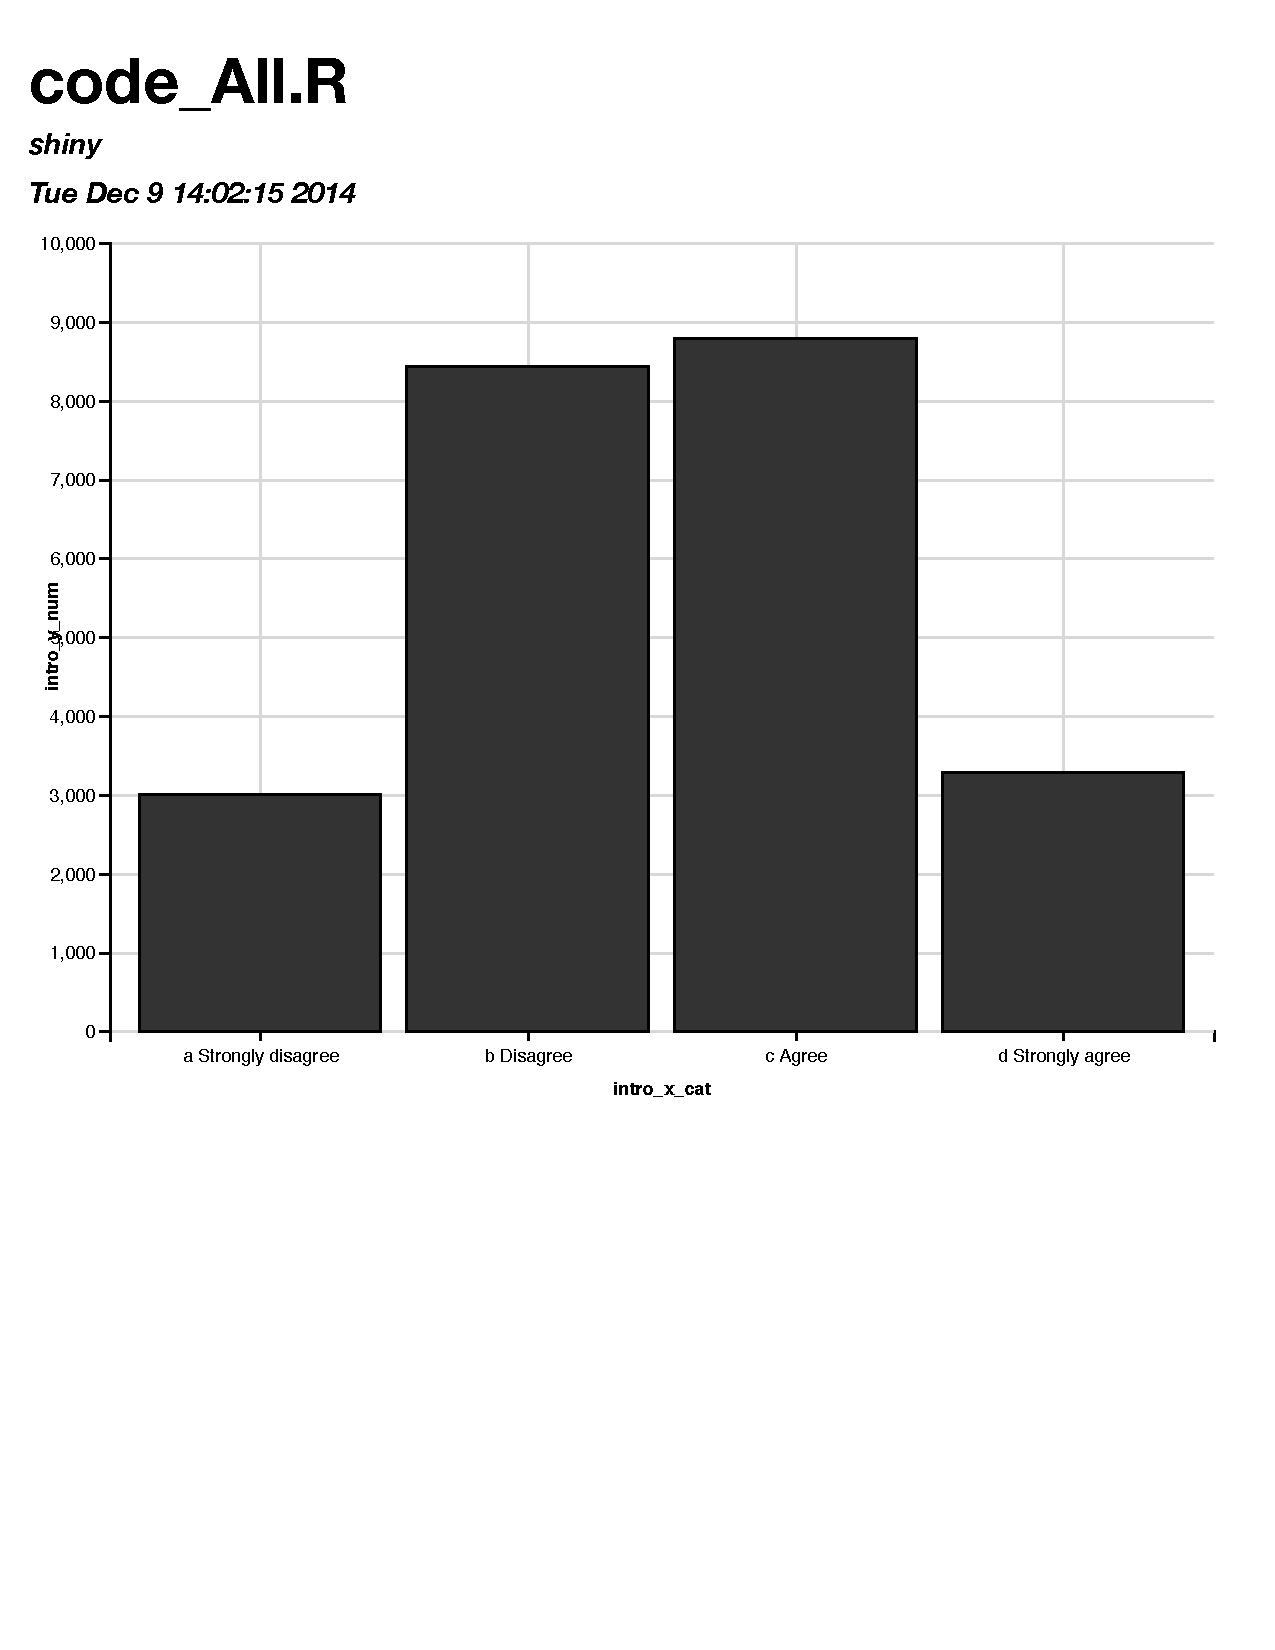
\includegraphics[width=2.5in]{barchart.pdf}}

\item {\em (5pts)} Make a summary of the Enjoy.Maths variable. What proportion of these students agree or strongly agree with the statement ``I enjoy mathematics"?

\begin{tabular}{lrr}
Category & Count & Proportion \\\hline
Strongly disagree & 2074 & 0.131\\
Disagree & 5776 & 0.365 \\
Agree & 5820 &0.368 \\
Strongly Agree & 2161 & 0.137\\
\end{tabular}

{\em 0.50 say they agree or strongly agree.}

\item Use the Intro Stats app to obtain a contingency table and mosaic plot of the relationship between Country (X, Factor) and Enjoy.Maths (Y, Response).  
{\em (5pts)} Print contingency tables with the {\bf Count} and {\bf Column \%} values.  Print out the output and turn it in with this assignment. \\

\centerline{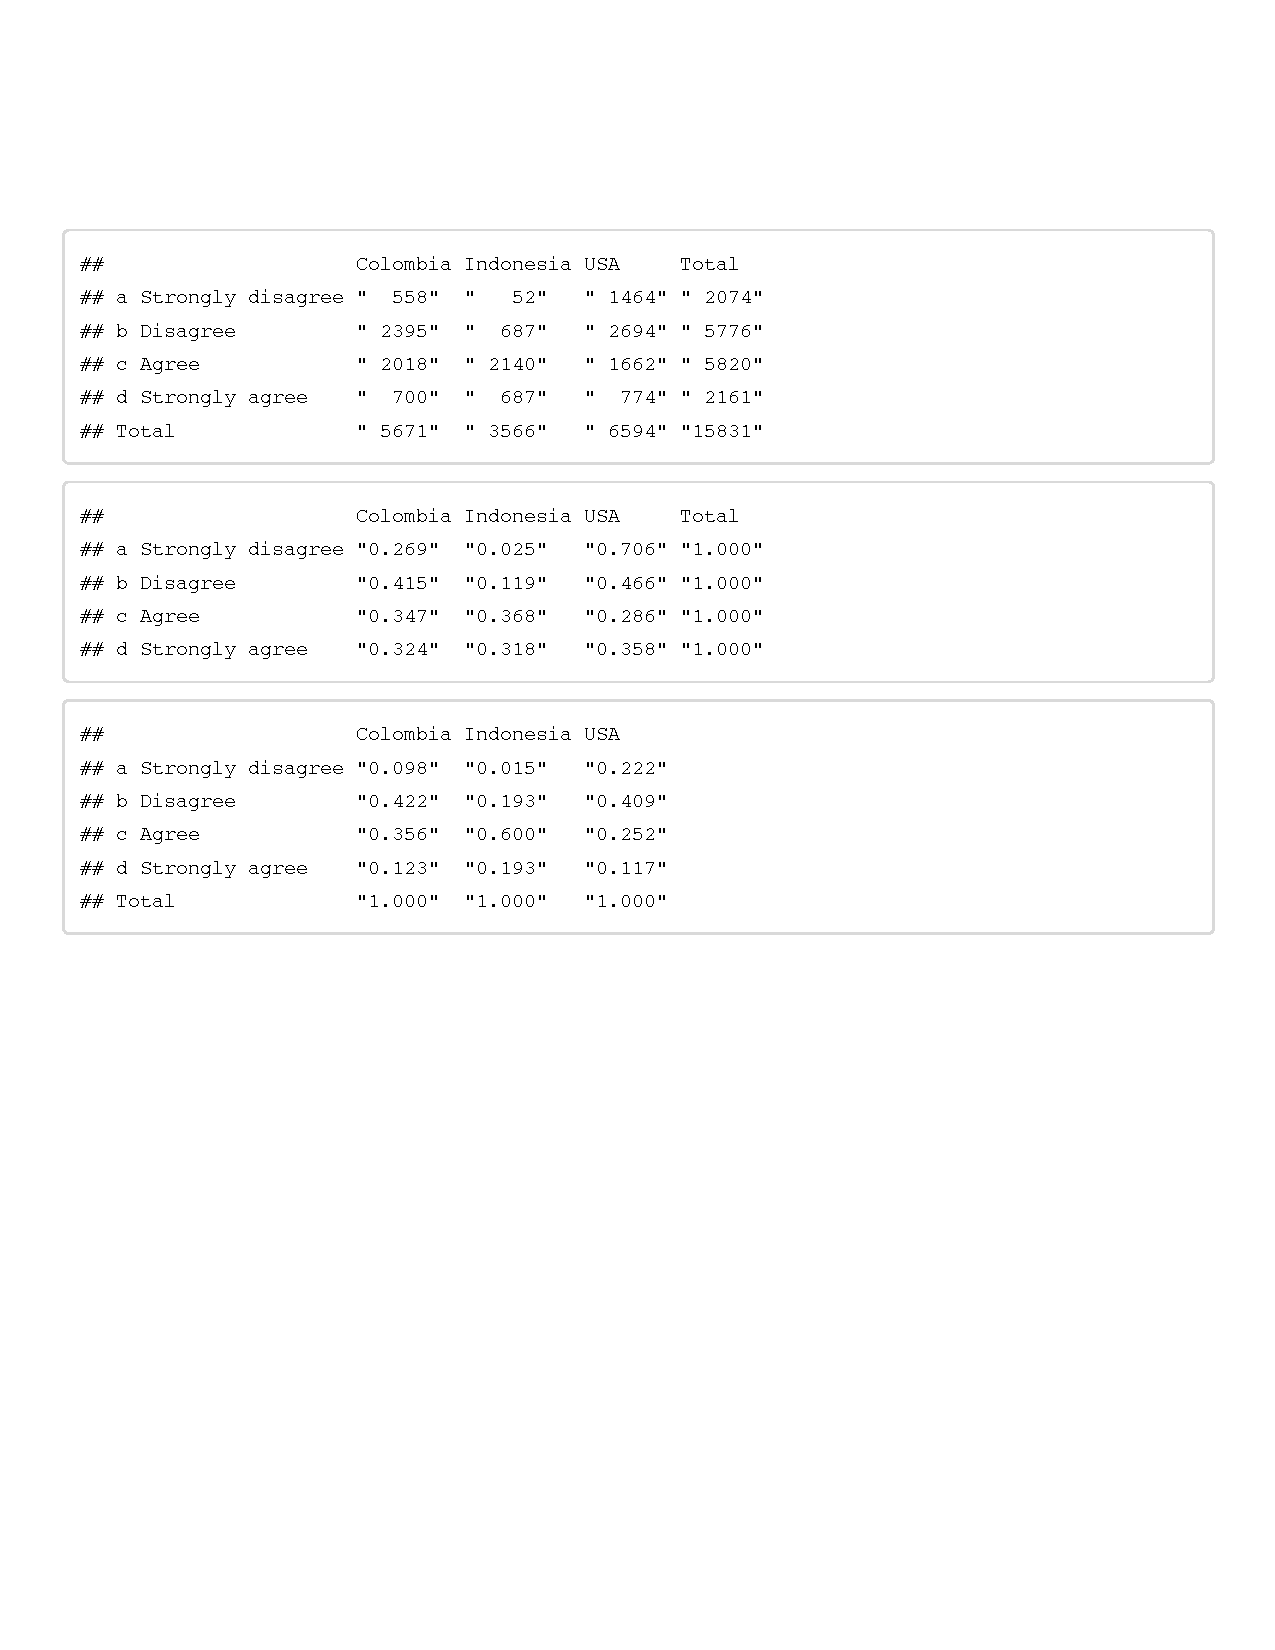
\includegraphics[width=5in]{contingency.pdf}}

\centerline{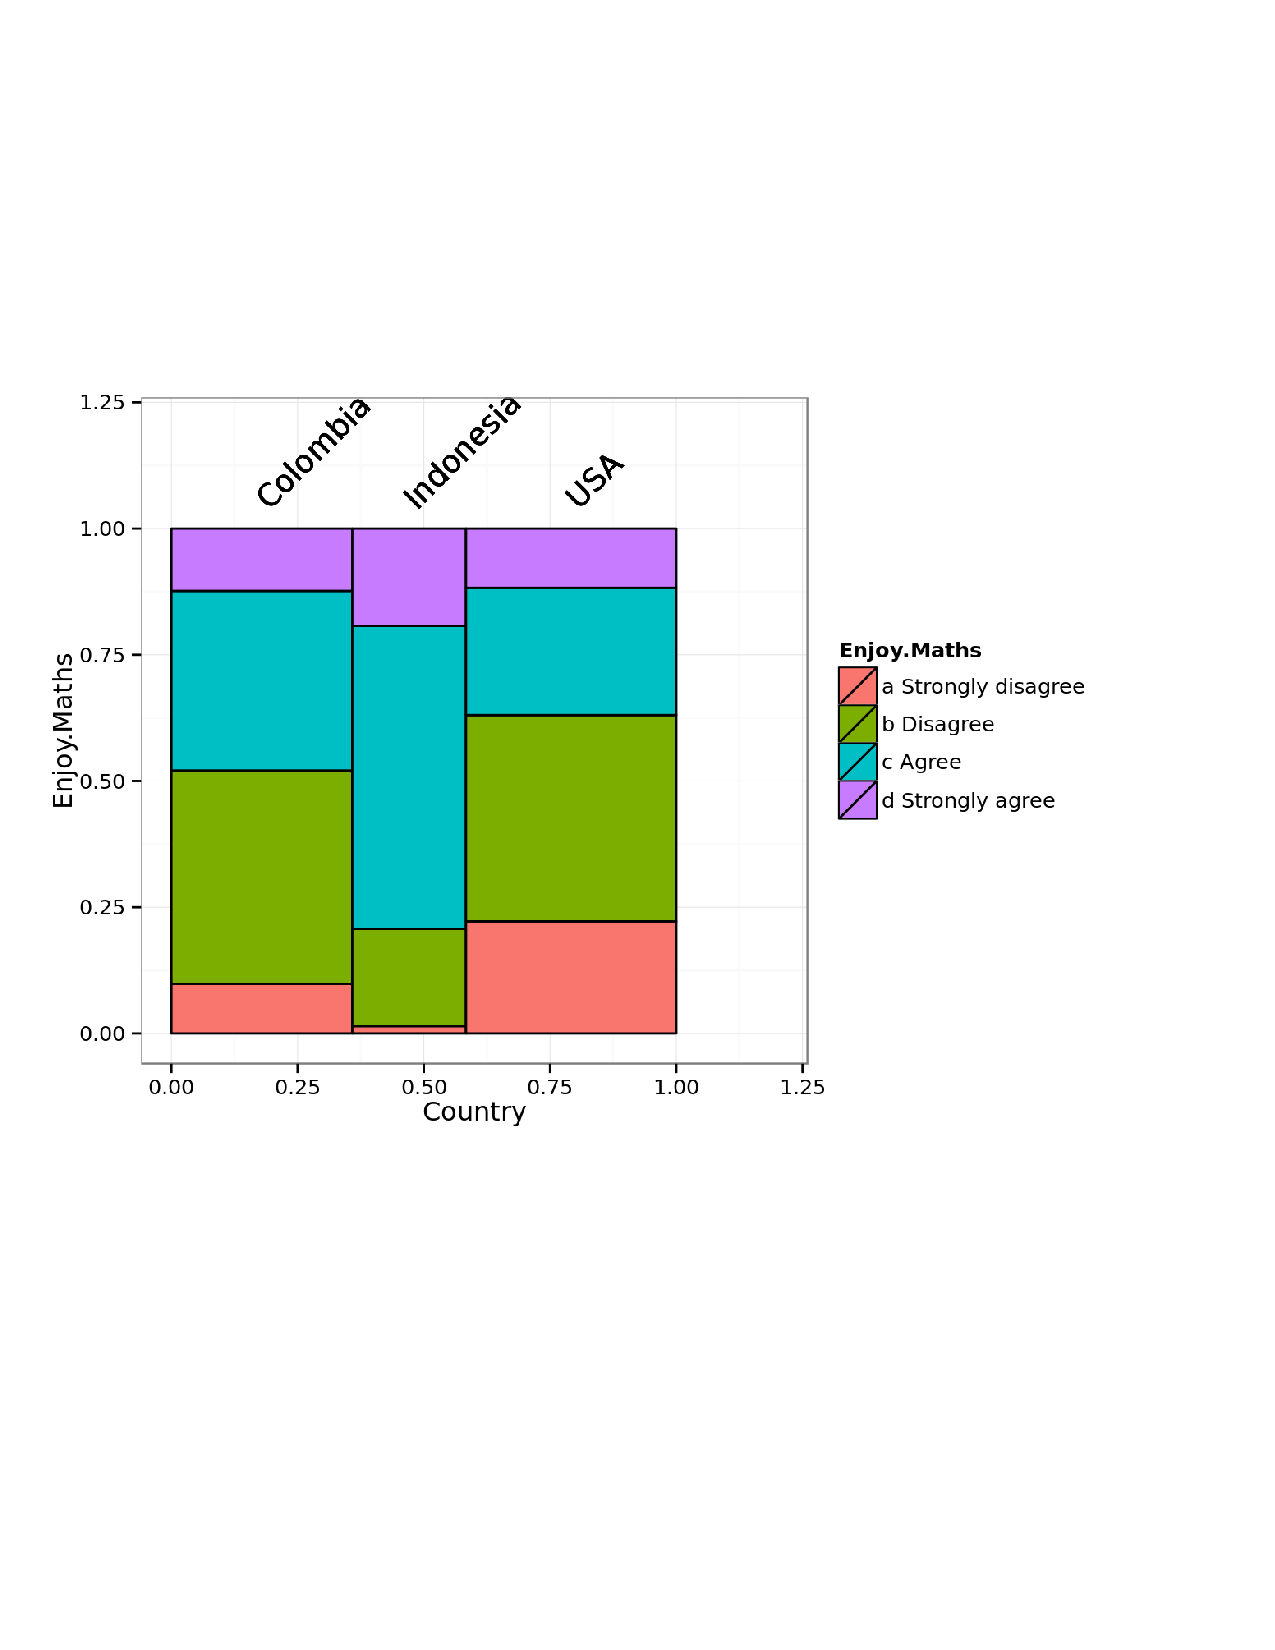
\includegraphics[width=4in]{mosaic.pdf}}

\item {\em (2pts)} Explain the meaning of the number {\bf 52} from the contingency table of counts.

{\em This is the number of students in Indonesia who Strongly disagreed with the statement ``I enjoy mathematics".}

\item {\em (3pts)} Give the conditional distribution of ``Strongly agree'' given the Country. 

{\em Conditional on country the values for strongly disagree are 0.123,  0.193, 0.117.}  

\item {\em (2pts)} Compare this conditional distribution to the overall marginal distribution of ``Strongly Agree". 

{\em Overall the proportions that strongly agree is 0.137. Indonesia has a bigger proportion that agree than we would expect if all countries were the same.}

\item {\em (3pts)} Based on the contingency table and mosaic plot, does it appear there is an association between whether students report enjoying math and the country in which they attend school?  Circle the appropriate answer below.  Then given an explanation for your answer.

{\em Yes, there is an association}

Explain your answer:

{\em The proportions for the different responses are quite different from one country to another, which indicates the association. Students in Indonesia tend to more often report that they agree with the statement ``I enjoy mathematics", than either Colombia or the USA. }

\end{enumerate}

\end{document}